\subsection{Técnica de Townsend pulsada}

Para estudiar el transporte de electrones en una mezcla gaseosa se utilizó
un aparato de Townsend pulsado, cuyo esquema se presenta en la
Fig.~\ref{fig:camara-townsend}. El sistema estaba constituido por una cámara
con dos electrodos planos y paralelos separados una distancia
\(d=3.0~\mathrm{cm}\), una fuente de alto voltaje, un láser ultravioleta,
un fotodiodo, un amplificador corriente--voltaje, un osciloscopio y un
sistema de adquisición controlado mediante computadora.\\

\begin{figure}
    \centering
    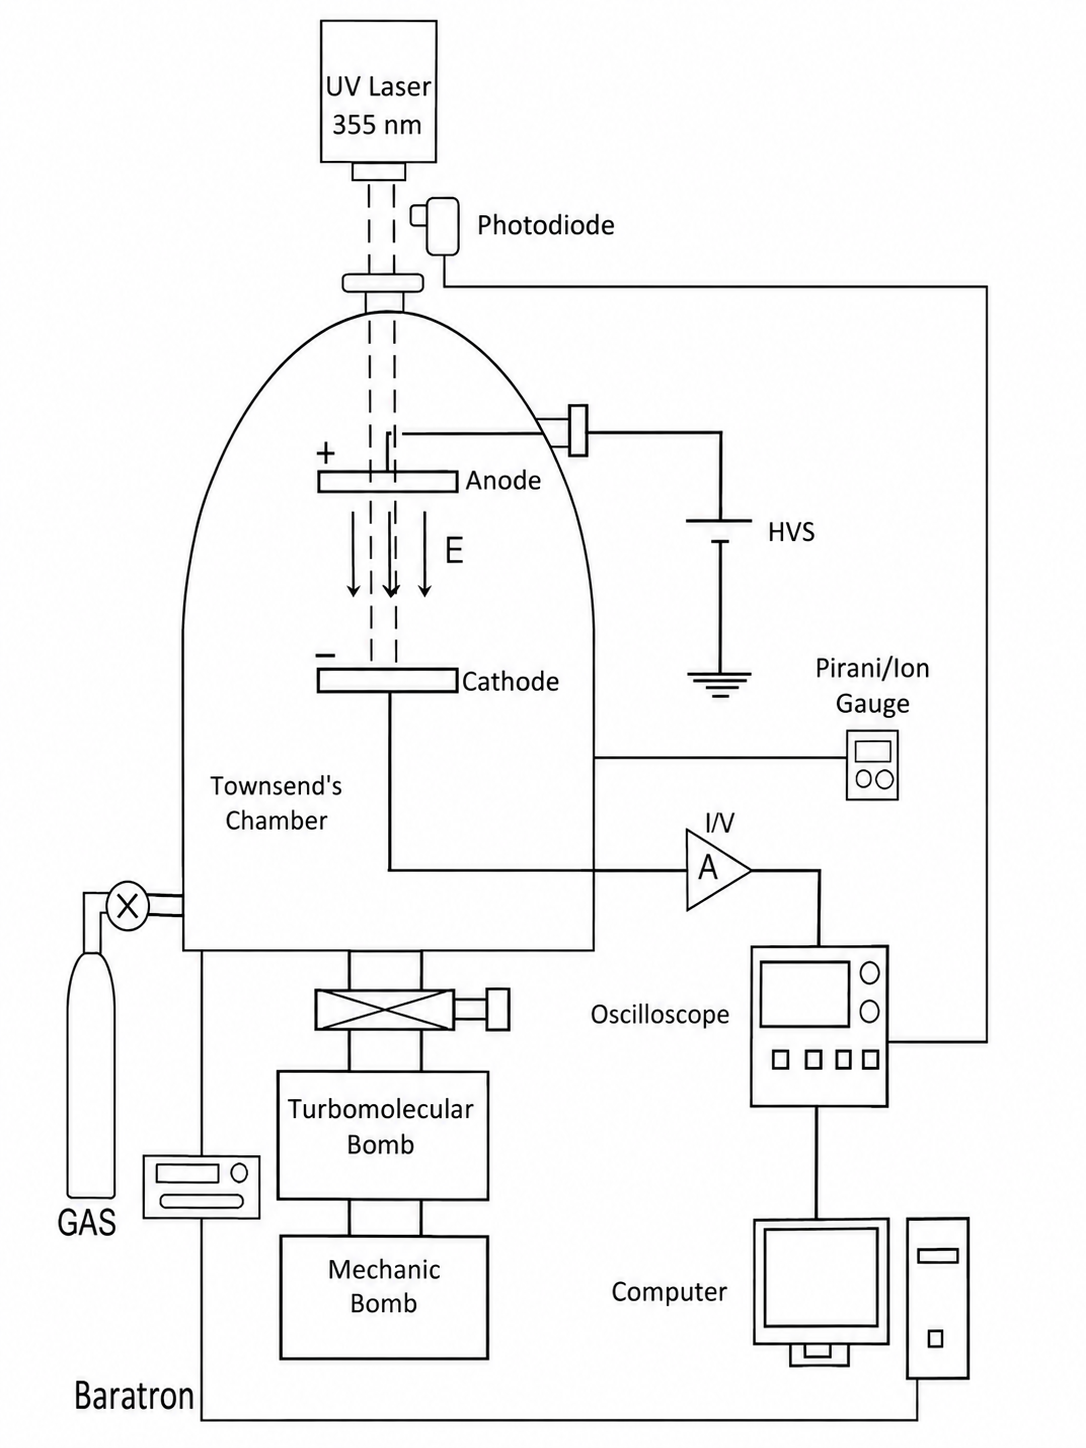
\includegraphics[width=\columnwidth]{figuras/chamber.png}
    \captionof{figure}{Diagrama del aparato de Townsend pulsado utilizado
    para medir la corriente electrónica transitoria.}
    \label{fig:camara-townsend}
\end{figure}

La cámara se encontraba conectada a una bomba mecánica y a una bomba
turbomolecular. Antes de introducir el gas se evacuó la cámara mediante la bomba mecanica y despues la turbomolecular, hasta alcanzar una presión base del orden de
\(2.5\times10^{-6}~\mathrm{Torr}\). Este procedimiento permitió reducir la
presencia de aire, vapor de agua y residuos de gases empleados previamente.
Posteriormente, se introdujo una mezcla compuesta por \(1\%\) de nitrógeno
y \(99\%\) de argón. Las mediciones se realizaron para diferentes presiones
de trabajo, comprendidas aproximadamente entre \(10.1\) y
\(200~\mathrm{Torr}\).\\

Entre los electrodos se aplicó una diferencia de potencial \(V\), con la
cual se produjo un campo eléctrico $E$ aproximadamente uniforme, las condiciones experimentales se caracterizaron mediante
el campo eléctrico reducido $E/N$ (donde $N$ es la densidad numerica del gas), expresado en unidades townsend, donde
\(1~\mathrm{Td}=10^{-21}~\mathrm{V\,m^{2}}\). El software del laboratorio
utilizó la presión, la temperatura y la separación entre los electrodos
para establecer el voltaje requerido para cada valor seleccionado de
\(E/N\).\\

Los electrones iniciales se produjeron al hacer incidir pulsos de un láser
ultravioleta de \(355~\mathrm{nm}\) sobre el cátodo. La intensidad de los
pulsos se reguló mediante un polarizador y mediante los controles del
sistema, con el propósito de obtener una señal medible sin saturar los
instrumentos ni producir descargas sostenidas. El fotodiodo detectó cada
pulso láser y proporcionó la referencia temporal utilizada para sincronizar
el osciloscopio.\\

Una vez liberados del cátodo, los electrones se desplazaron hacia el ánodo
bajo la acción del campo eléctrico y produjeron una corriente electrónica
transitoria. La corriente producida dentro de la cámara se
condujo hacia un amplificador \(I/V\), cuya señal de salida se registró con
el osciloscopio.\\

Las señales registradas en el osciloscopio presentaron una subida inicial abrupta,
seguida por una región monotona creciente y una caída asociada con
el final de la componente electrónica, como se representa
 en la Fig.~\ref{fig:transitorio-electronico}. Mediante los
cursores del osciloscopio se fijó el origen temporal \(t_0\) en el comienzo
de la subida de la señal. Como criterio operativo, el tiempo de tránsito
electrónico \(t_{\mathrm e}\) se definió como el intervalo entre \(t_0\) y
el punto medio de la caída final, el cual se estimo visualmente en la pantalla del osciloscopio.\\

\begin{figure}
    \centering
    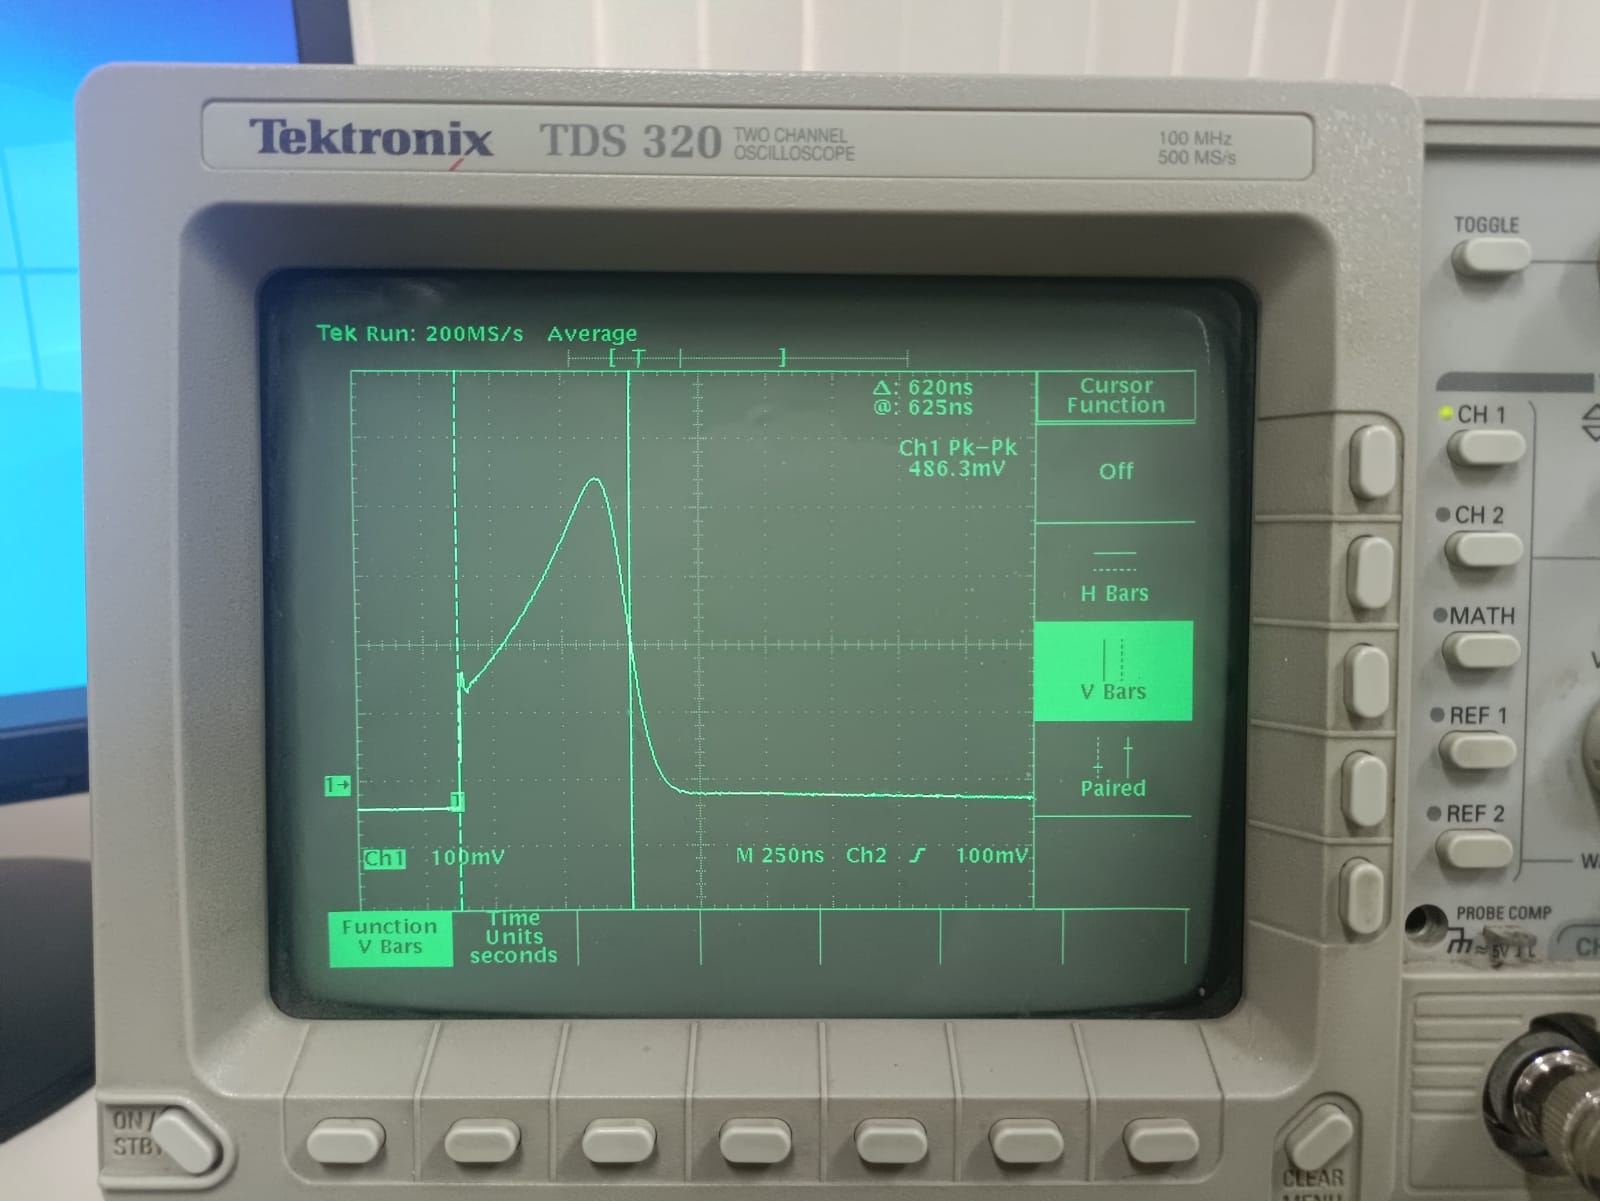
\includegraphics[width=0.75\columnwidth]
    {figuras/oz.jpeg}
    \caption{Señal electrónica transitoria
    observada en el osciloscopio. El origen temporal \(t_0\) se fijó en el
    inicio de la subida, mientras que el tiempo de tránsito \(t_{\mathrm e}\)
    se determinó en el punto medio de la caída final.}
    \label{fig:transitorio-electronico}
\end{figure}

A partir del tiempo medido se calculó la velocidad de deriva mediante $v_{\mathrm d}=\frac{d}{t_{\mathrm e}}$, 
donde \(d=3.0~\mathrm{cm}\) fue la separación entre los electrodos. El procedimiento se repitió para diferentes valores de presión y de campo
eléctrico reducido. El sistema de adquisición registró para cada medición
la presión, la temperatura, el voltaje aplicado, el valor de \(E/N\) y las
escalas empleadas en el osciloscopio. El barrido se interrumpió cuando se observaron descargas entre los
electrodos y las paredes de la cámara. En consecuencia, el valor máximo de
\(E/N\) alcanzado no fue el mismo para todas las presiones. Las mediciones
posteriores al inicio de estas descargas no se consideraron en el análisis,
pues ya no correspondían al régimen de corriente electrónica transitoria
empleado para determinar el tiempo de tránsito.\\

Finalmente, las velocidades obtenidas
se representaron en función de \(E/N\), lo que permitió comparar las
mediciones realizadas bajo distintas condiciones de presión.\\


